\documentclass[11pt,]{article}
\usepackage{lmodern}
\usepackage{amssymb,amsmath}
\usepackage{ifxetex,ifluatex}
\usepackage{fixltx2e} % provides \textsubscript
\ifnum 0\ifxetex 1\fi\ifluatex 1\fi=0 % if pdftex
  \usepackage[T1]{fontenc}
  \usepackage[utf8]{inputenc}
\else % if luatex or xelatex
  \ifxetex
    \usepackage{mathspec}
  \else
    \usepackage{fontspec}
  \fi
  \defaultfontfeatures{Ligatures=TeX,Scale=MatchLowercase}
\fi
% use upquote if available, for straight quotes in verbatim environments
\IfFileExists{upquote.sty}{\usepackage{upquote}}{}
% use microtype if available
\IfFileExists{microtype.sty}{%
\usepackage{microtype}
\UseMicrotypeSet[protrusion]{basicmath} % disable protrusion for tt fonts
}{}
\usepackage[margin = 1.5in]{geometry}
\usepackage{hyperref}
\PassOptionsToPackage{usenames,dvipsnames}{color} % color is loaded by hyperref
\hypersetup{unicode=true,
            pdftitle={Optimization: Part 1},
            pdfauthor={Abhinav Anand, IIMB},
            colorlinks=true,
            linkcolor=blue,
            citecolor=magenta,
            urlcolor=red,
            breaklinks=true}
\urlstyle{same}  % don't use monospace font for urls
\usepackage{color}
\usepackage{fancyvrb}
\newcommand{\VerbBar}{|}
\newcommand{\VERB}{\Verb[commandchars=\\\{\}]}
\DefineVerbatimEnvironment{Highlighting}{Verbatim}{commandchars=\\\{\}}
% Add ',fontsize=\small' for more characters per line
\usepackage{framed}
\definecolor{shadecolor}{RGB}{248,248,248}
\newenvironment{Shaded}{\begin{snugshade}}{\end{snugshade}}
\newcommand{\KeywordTok}[1]{\textcolor[rgb]{0.13,0.29,0.53}{\textbf{#1}}}
\newcommand{\DataTypeTok}[1]{\textcolor[rgb]{0.13,0.29,0.53}{#1}}
\newcommand{\DecValTok}[1]{\textcolor[rgb]{0.00,0.00,0.81}{#1}}
\newcommand{\BaseNTok}[1]{\textcolor[rgb]{0.00,0.00,0.81}{#1}}
\newcommand{\FloatTok}[1]{\textcolor[rgb]{0.00,0.00,0.81}{#1}}
\newcommand{\ConstantTok}[1]{\textcolor[rgb]{0.00,0.00,0.00}{#1}}
\newcommand{\CharTok}[1]{\textcolor[rgb]{0.31,0.60,0.02}{#1}}
\newcommand{\SpecialCharTok}[1]{\textcolor[rgb]{0.00,0.00,0.00}{#1}}
\newcommand{\StringTok}[1]{\textcolor[rgb]{0.31,0.60,0.02}{#1}}
\newcommand{\VerbatimStringTok}[1]{\textcolor[rgb]{0.31,0.60,0.02}{#1}}
\newcommand{\SpecialStringTok}[1]{\textcolor[rgb]{0.31,0.60,0.02}{#1}}
\newcommand{\ImportTok}[1]{#1}
\newcommand{\CommentTok}[1]{\textcolor[rgb]{0.56,0.35,0.01}{\textit{#1}}}
\newcommand{\DocumentationTok}[1]{\textcolor[rgb]{0.56,0.35,0.01}{\textbf{\textit{#1}}}}
\newcommand{\AnnotationTok}[1]{\textcolor[rgb]{0.56,0.35,0.01}{\textbf{\textit{#1}}}}
\newcommand{\CommentVarTok}[1]{\textcolor[rgb]{0.56,0.35,0.01}{\textbf{\textit{#1}}}}
\newcommand{\OtherTok}[1]{\textcolor[rgb]{0.56,0.35,0.01}{#1}}
\newcommand{\FunctionTok}[1]{\textcolor[rgb]{0.00,0.00,0.00}{#1}}
\newcommand{\VariableTok}[1]{\textcolor[rgb]{0.00,0.00,0.00}{#1}}
\newcommand{\ControlFlowTok}[1]{\textcolor[rgb]{0.13,0.29,0.53}{\textbf{#1}}}
\newcommand{\OperatorTok}[1]{\textcolor[rgb]{0.81,0.36,0.00}{\textbf{#1}}}
\newcommand{\BuiltInTok}[1]{#1}
\newcommand{\ExtensionTok}[1]{#1}
\newcommand{\PreprocessorTok}[1]{\textcolor[rgb]{0.56,0.35,0.01}{\textit{#1}}}
\newcommand{\AttributeTok}[1]{\textcolor[rgb]{0.77,0.63,0.00}{#1}}
\newcommand{\RegionMarkerTok}[1]{#1}
\newcommand{\InformationTok}[1]{\textcolor[rgb]{0.56,0.35,0.01}{\textbf{\textit{#1}}}}
\newcommand{\WarningTok}[1]{\textcolor[rgb]{0.56,0.35,0.01}{\textbf{\textit{#1}}}}
\newcommand{\AlertTok}[1]{\textcolor[rgb]{0.94,0.16,0.16}{#1}}
\newcommand{\ErrorTok}[1]{\textcolor[rgb]{0.64,0.00,0.00}{\textbf{#1}}}
\newcommand{\NormalTok}[1]{#1}
\usepackage{graphicx,grffile}
\makeatletter
\def\maxwidth{\ifdim\Gin@nat@width>\linewidth\linewidth\else\Gin@nat@width\fi}
\def\maxheight{\ifdim\Gin@nat@height>\textheight\textheight\else\Gin@nat@height\fi}
\makeatother
% Scale images if necessary, so that they will not overflow the page
% margins by default, and it is still possible to overwrite the defaults
% using explicit options in \includegraphics[width, height, ...]{}
\setkeys{Gin}{width=\maxwidth,height=\maxheight,keepaspectratio}
\IfFileExists{parskip.sty}{%
\usepackage{parskip}
}{% else
\setlength{\parindent}{0pt}
\setlength{\parskip}{6pt plus 2pt minus 1pt}
}
\setlength{\emergencystretch}{3em}  % prevent overfull lines
\providecommand{\tightlist}{%
  \setlength{\itemsep}{0pt}\setlength{\parskip}{0pt}}
\setcounter{secnumdepth}{0}
% Redefines (sub)paragraphs to behave more like sections
\ifx\paragraph\undefined\else
\let\oldparagraph\paragraph
\renewcommand{\paragraph}[1]{\oldparagraph{#1}\mbox{}}
\fi
\ifx\subparagraph\undefined\else
\let\oldsubparagraph\subparagraph
\renewcommand{\subparagraph}[1]{\oldsubparagraph{#1}\mbox{}}
\fi

%%% Use protect on footnotes to avoid problems with footnotes in titles
\let\rmarkdownfootnote\footnote%
\def\footnote{\protect\rmarkdownfootnote}

%%% Change title format to be more compact
\usepackage{titling}

% Create subtitle command for use in maketitle
\newcommand{\subtitle}[1]{
  \posttitle{
    \begin{center}\large#1\end{center}
    }
}

\setlength{\droptitle}{-2em}

  \title{Optimization: Part 1}
    \pretitle{\vspace{\droptitle}\centering\huge}
  \posttitle{\par}
    \author{Abhinav Anand, IIMB}
    \preauthor{\centering\large\emph}
  \postauthor{\par}
      \predate{\centering\large\emph}
  \postdate{\par}
    \date{2018/07/05}

\linespread{1.25}
\usepackage{amsmath}

\begin{document}
\maketitle

\section{Background}\label{background}

Problems in finance and economics are often concerned with the behavior
of agents who are considered to be utility maximizers. Utility functions
are thought to be monotonic in their variables---more of a utility
enhancing variable is better than less---and are thought to obey
diminishing returns as the variables scale.\footnote{This utility
  function can assume a variety of forms. For example, if the `agent' is
  a firm, its utility is its profit function; if it's a government, it
  could be some (aggregate) social welfare function etc.} Additionally,
real-life constraints ensure that variables are bounded. Hence
optimization of functions under constraints forms an important
discipline in the study of such subjects.

After linear optimization, quadratic optimization problems are the
simplest since they can be captured in \emph{quadratic forms} and can be
represented via symmetric matrices with special properties. A
distinguishing feature of quadratic optimization is the presence of
first and second order conditions that characterize the nature of the
extreme point.

\subsection{Quadratic Optimization}\label{quadratic-optimization}

In one dimension, \(x\in \mathbb{R}\) the simplest quadratic objective
functions can be \(f(x)=\{x^2, -x^2\}\) with the first attaining a
global minimum and the second a global maximum at \(x=0\).

\begin{Shaded}
\begin{Highlighting}[]
\NormalTok{x <-}\StringTok{ }\OperatorTok{-}\DecValTok{500}\OperatorTok{:}\DecValTok{500}
\NormalTok{y_}\DecValTok{1}\NormalTok{ <-}\StringTok{ }\NormalTok{x}\OperatorTok{^}\DecValTok{2}
\NormalTok{y_}\DecValTok{2}\NormalTok{ <-}\StringTok{ }\OperatorTok{-}\NormalTok{x}\OperatorTok{^}\DecValTok{2}
\NormalTok{data_l <-}\StringTok{ }\KeywordTok{cbind}\NormalTok{(x, y_}\DecValTok{1}\NormalTok{, y_}\DecValTok{2}\NormalTok{) }\OperatorTok\StringTok{ }
\StringTok{  }\NormalTok{dplyr}\OperatorTok{::}\KeywordTok{as_tibble}\NormalTok{() }\OperatorTok\StringTok{ }\CommentTok{#wide format}
\StringTok{  }\NormalTok{tidyr}\OperatorTok{::}\KeywordTok{gather}\NormalTok{(., }
\NormalTok{                y_}\DecValTok{1}\OperatorTok{:}\NormalTok{y_}\DecValTok{2}\NormalTok{, }
                \DataTypeTok{key =} \StringTok{'y'}\NormalTok{, }
                \DataTypeTok{value =} \StringTok{'f'}\NormalTok{) }\CommentTok{#long format}

\KeywordTok{ggplot}\NormalTok{(data_l, }\KeywordTok{aes}\NormalTok{(x, f, }\DataTypeTok{color =}\NormalTok{ y)) }\OperatorTok{+}
\StringTok{  }\KeywordTok{geom_line}\NormalTok{() }\OperatorTok{+}
\StringTok{  }\KeywordTok{geom_hline}\NormalTok{(}\DataTypeTok{yintercept =} \DecValTok{0}\NormalTok{) }\OperatorTok{+}
\StringTok{  }\KeywordTok{theme_minimal}\NormalTok{()}
\end{Highlighting}
\end{Shaded}

\begin{center}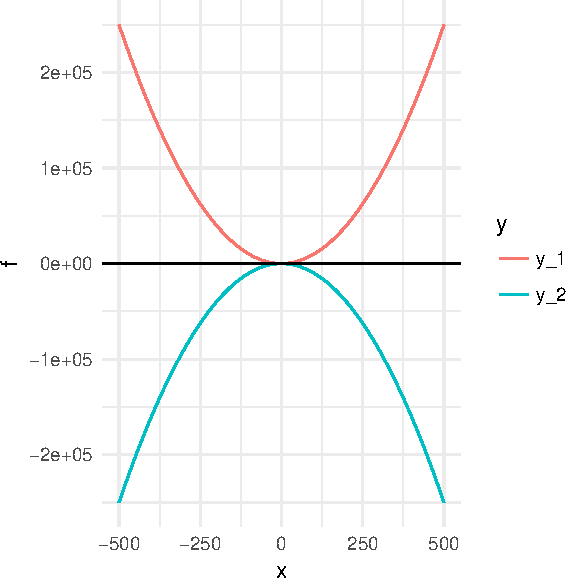
\includegraphics{Optimization_files/figure-latex/opt_dim_1-1} \end{center}

\subsubsection{Quadratic Forms}\label{quadratic-forms}

For the case when \(x = (x_1, x_2) \in \mathbb{R}^2\), a general
quadratic form is the following: \[
Q(x) = a_{11}x_1^2 + a_{22}x_2^2 + 2a_{12}x_1x_2
\] which may be represented as a matrix: \[
Q(x) = [x_1 x_2]\begin{bmatrix}a_{11} & a_{12}\\ a_{12} & a_{22}\end{bmatrix}
\begin{bmatrix}x_1 \\ x_2\end{bmatrix}
\] Similarly, when \(x = (x_1, x_2, x_3) \in \mathbb{R}^3\), the form
becomes \[
Q(x) = [x_1 x_2 x_3]\begin{bmatrix}a_{11} & a_{12} & a_{13}\\ a_{12} & a_{22} & a_{23}\\
a_{13} & a_{23} & a_{33}\end{bmatrix} \begin{bmatrix}x_1 \\ x_2 \\ x_3\end{bmatrix}
\] and in general, when \(x = (x_1, \hdots, x_n) \in \mathbb{R}^n\): \[
Q(x) = [x_1 \hdots x_n]\begin{bmatrix}a_{11} & \hdots & a_{1n}\\ \vdots\\
a_{1n} & \hdots & a_{nn}\end{bmatrix} \begin{bmatrix}x_1\\ \vdots\\ x_n\end{bmatrix}
\] It's easy to see that \(Q(0) = 0\). If \(a>0, ax^2>0\) and we can
call the quadratic form ``positive definite''. Similarly, if
\(a<0, ax^2<0\) and we call the form ``negative definite''. This carries
over when \(x\in \mathbb{R}^2\), since \(Q(x_1, x_2) = x_1^2+x_2^2>0\)
(positive definite) and \(Q(x_1, x_2) = -x_1^2-x_2^2>0\) (negative
definite). Additionally for the case when
\(Q(x_1, x_2) = x_1^2-x_2^2>0\), the quadratic form is
\emph{indefinite}.

In general, symmetric matrices are called positive (semi)definite,
negative (semi)definite etc. according to the definiteness of the
expression \(Q(x) = x^{\top}Ax\).\footnote{Hence if
  \(\forall x\neq0\in \mathbb{R}^n, x^{\top}Ax\geq 0\) the form is
  positive semidefinite and so on.} Additionally for symmetric matrices,
the eigenvalues are all real numbers. A highly useful fact to know is
that for positive definite matrices, all eigenvalues are positive; for
negative definite matrices, all eigenvalues are negative; and for
indefinite matrices, some eigenvalues are positive and some are
negative.

\section{Quadratic Programming}\label{quadratic-programming}

In general, a quadratic programming problem can assume the following
form: \[\min{} \frac{1}{2}x^{\top}Dx-d^{\top}x:\] \[Ex = c\]
\[A^{\top}x\geq b\] \[x\geq 0\]

Constraints must be linear and the objective must be quadratic. Without
loss of generality, the matrix \(D\) may be assumed symmetric. However
it must be positive semidefinite.

\subsection{Computation: Quadratic
Programming}\label{computation-quadratic-programming}

The package \texttt{quadprog} includes subroutines for solving quadratic
programming problems. We use the function \texttt{solve.QP()} for this
purpose.

The general syntax for solving such quadratic programming problems is
the following:

\begin{Shaded}
\begin{Highlighting}[]
\NormalTok{quadprog}\OperatorTok{::}\KeywordTok{solve.QP}\NormalTok{(}\DataTypeTok{Dmat =}\NormalTok{ ..., }\CommentTok{#the D matrix of quadratic coefficients}
                   \DataTypeTok{dvec =}\NormalTok{ ..., }\CommentTok{#the d vector}
                   \DataTypeTok{Amat =}\NormalTok{ ..., }\CommentTok{#the constraint matrix}
                   \DataTypeTok{bvec =}\NormalTok{ ... }\CommentTok{#the constraint RHS}
                   \DataTypeTok{meq =} \DecValTok{0}\NormalTok{, }\CommentTok{#how many first few equality constraints}
\NormalTok{                  )}
\end{Highlighting}
\end{Shaded}

We quote from the documentation for the function \texttt{solve.QP()}

\begin{quote}
Description
\end{quote}

\begin{quote}
This routine implements the dual method of Goldfarb and Idnani (1982,
1983) for solving quadratic programming problems of the form min(-d\^{}T
b + 1/2 b\^{}T D b) with the constraints A\^{}T b \textgreater{}= b\_0.
\end{quote}

Hence keeping in mind the factor 1/2 in the objective function and the
fact that one needs to specify \(A^{\top}\) for the matrix constraint,
we are ready to solve quadratic programs.

\textbf{Illustration:} Solve the following quadratic program:
\[\min f(x)=1/2x_1^2+x_2^2-x_1x_2-2x_1-6x_2:\] \[x_1+x_2\leq 2\]
\[-x_1+2x_2\leq 2\] \[2x_1+x_2\leq 3\] \[x_1, x_2\geq 0\]

This problem may be rewritten in matrix form:
\[\min{} \frac{1}{2}[x_1,x_2]\begin{bmatrix}1,-1\\-1,2\end{bmatrix}
\begin{bmatrix}x_1\\x_2\end{bmatrix}-[2,6]\begin{bmatrix}x_1\\x_2\end{bmatrix}:\]
\[\begin{bmatrix}
-1, -1\\
1, -2\\
-2, -1\\
\end{bmatrix}
\begin{bmatrix}
x_1\\
x_2
\end{bmatrix}\geq
\begin{bmatrix}
-2\\
-2\\
-3
\end{bmatrix}\]

We can solve this quadratic program via the following:

\begin{Shaded}
\begin{Highlighting}[]
\NormalTok{Dmat <-}\StringTok{ }\KeywordTok{matrix}\NormalTok{(}\KeywordTok{c}\NormalTok{(}\DecValTok{1}\NormalTok{,}\OperatorTok{-}\DecValTok{1}\NormalTok{,}\OperatorTok{-}\DecValTok{1}\NormalTok{,}\DecValTok{2}\NormalTok{),}\DecValTok{2}\NormalTok{,}\DecValTok{2}\NormalTok{)}
\NormalTok{dvec =}\StringTok{ }\KeywordTok{c}\NormalTok{(}\DecValTok{2}\NormalTok{,}\DecValTok{6}\NormalTok{)}
\NormalTok{Amat =}\StringTok{ }\KeywordTok{matrix}\NormalTok{(}\KeywordTok{c}\NormalTok{(}\OperatorTok{-}\DecValTok{1}\NormalTok{,}\OperatorTok{-}\DecValTok{1}\NormalTok{,}\DecValTok{1}\NormalTok{,}\OperatorTok{-}\DecValTok{2}\NormalTok{,}\OperatorTok{-}\DecValTok{2}\NormalTok{,}\OperatorTok{-}\DecValTok{1}\NormalTok{),}\DecValTok{2}\NormalTok{,}\DecValTok{3}\NormalTok{)}
\NormalTok{bvec =}\StringTok{ }\KeywordTok{c}\NormalTok{(}\OperatorTok{-}\DecValTok{2}\NormalTok{,}\OperatorTok{-}\DecValTok{2}\NormalTok{,}\OperatorTok{-}\DecValTok{3}\NormalTok{)}

\NormalTok{quadprog}\OperatorTok{::}\KeywordTok{solve.QP}\NormalTok{(Dmat, dvec, Amat, bvec)}
\end{Highlighting}
\end{Shaded}

\begin{verbatim}
## $solution
## [1] 0.6666667 1.3333333
## 
## $value
## [1] -8.222222
## 
## $unconstrained.solution
## [1] 10  8
## 
## $iterations
## [1] 3 0
## 
## $Lagrangian
## [1] 3.1111111 0.4444444 0.0000000
## 
## $iact
## [1] 1 2
\end{verbatim}

\subsection{Application: Mean-Variance
Optimization}\label{application-mean-variance-optimization}

A classic application of quadratic programming is its use in
mean-variance optimization for portfolios. We illustrate it with the
following example:

Suppose an investor has \(n\) assets in her portfolio. She wishes to
find best weights for each portfolio. She likes high returns but also
wants low risk.

She could frame this problem as one about minimizing the variance of the
portfolio while subjecting returns to a certain lower bound.\footnote{Risk
  is often assumed to be (roughly) measurable via the variation in a
  security's prices---hence variance. Volatility is the name for the
  standard deviation. The idea is that securities with more price
  fluctuations, and hence more variance, are more risky.} Suppose she
possesses securities with returns according to normal random variables
\(X_i\sim \mathcal{N}(\mu_i, \sigma_i)\); and has apportioned fractional
weights \(w_i\) for each of them.

Then for two securities:

\[P_2 \sim \mathcal{N}(w_1\mu_1+w_2\mu_2; w_1^2\sigma_1^2+w_2^2\sigma_2^2+2w_1w_2cov(X_1,X_2))\]

and for \(n\) securities in general:

\[P_n \sim \mathcal{N}(w^{\top}\mu; w^{\top}\Sigma w)\]

where \(\Sigma\) is the \(n\times n\) coavariance matrix.

Hence the optimization program for the investor becomes: minimize the
variance subject to the constraint that the return is higher than some
lower critical value.

\[\min{} w^{\top}\Sigma w:\]
\[w^{\top}\mu \geq \mu_*; w^{\top}e = 1; w\geq 0\]

This is of the same form as a quadratic program.

\textbf{Illustration:} Suppose there are two normally distributed common
stocks whose expected returns are \(\mu^{\top} = (1.8\%, 2.5\%)\) and
whose covariance matrix is:

\[\Sigma = 
\begin{bmatrix}
1.68, 0.34\\
0.34, 3.09\\
\end{bmatrix}
\]

Hence the minimization program is:

\[\min{} 1.68w_1^2+3.09w_2^2+2*0.34w_1w_2:\] \[w_1+w_2=1\]
\[0.018w_1 + 0.025w_2 \geq 0.018\] \[w_1, w_2\geq 0\]

\begin{Shaded}
\begin{Highlighting}[]
\NormalTok{D_mat <-}\StringTok{ }\KeywordTok{matrix}\NormalTok{(}\KeywordTok{c}\NormalTok{(}\FloatTok{1.68}\NormalTok{,}\FloatTok{0.34}\NormalTok{,}\FloatTok{0.34}\NormalTok{,}\FloatTok{3.09}\NormalTok{),}\DecValTok{2}\NormalTok{,}\DecValTok{2}\NormalTok{)}
\NormalTok{d_vec <-}\StringTok{ }\KeywordTok{c}\NormalTok{(}\DecValTok{0}\NormalTok{, }\DecValTok{0}\NormalTok{)}
\NormalTok{A_mat <-}\StringTok{ }\KeywordTok{matrix}\NormalTok{(}\KeywordTok{c}\NormalTok{(}\DecValTok{1}\NormalTok{,}\DecValTok{1}\NormalTok{,}\FloatTok{0.018}\NormalTok{,}\FloatTok{0.025}\NormalTok{), }\DataTypeTok{nrow =} \DecValTok{2}\NormalTok{, }\DataTypeTok{byrow =}\NormalTok{ F)}
\NormalTok{b_vec <-}\StringTok{ }\KeywordTok{c}\NormalTok{(}\DecValTok{1}\NormalTok{,}\FloatTok{0.018}\NormalTok{)}
\NormalTok{m_eq <-}\StringTok{ }\DecValTok{1}

\NormalTok{quadprog}\OperatorTok{::}\KeywordTok{solve.QP}\NormalTok{(D_mat, d_vec, A_mat, b_vec, m_eq)}
\end{Highlighting}
\end{Shaded}

\begin{verbatim}
## $solution
## [1] 0.6723716 0.3276284
## 
## $value
## [1] 0.620489
## 
## $unconstrained.solution
## [1] 0 0
## 
## $iterations
## [1] 2 0
## 
## $Lagrangian
## [1] 1.240978 0.000000
## 
## $iact
## [1] 1
\end{verbatim}

\section{Unconstrained Optimization}\label{unconstrained-optimization}

While it's clear what a maximum is in one dimension, what should be its
definition in two dimensions and beyond? The central idea remains the
same: \(x^*\) is the maximum if there is no other \(x\) in the domain of
\(f(x)\) such that \(f(x)\geq f(x^*)\). Note that this definition is
general and independent of the dimension of the underlying space from
where we pick \(x\). The only difference in dimensions one and beyond is
the structure of the domain; and while in one dimension it must take the
form \(x_L\leq x\leq x_H\), one needs such conditions for each component
when
\(x\in \mathbb{R}^n: x_{L1}\leq x_1\leq x_{H1}, \hdots, x_{Ln}\leq x_n\leq x_{Hn}\).
With this interpretation in mind, we are ready to formulate the
necessary and sufficient conditions for the optimal of an unconstrained
optimization program.

\subsection{First Order Conditions}\label{first-order-conditions}

When the dimension of the domain is 1, \(x_L\leq x\leq x_H\), the first
order condition stipulates that at the \emph{critical point} the
derivative be 0.\footnote{Why must this be so? Can you see the case for
  the plot \(f(x) = x^2\) and reason why?} Whether this critical point
is a (local) maximum or (local) minimum or neither, depends on the
\emph{second order condition} on the derivative of the derivative.

The example of \(f(x) = x^2\) illustrates this idea.

\begin{Shaded}
\begin{Highlighting}[]
\NormalTok{(plot_x_square <-}\StringTok{ }\KeywordTok{ggplot}\NormalTok{(}\DataTypeTok{data =}\NormalTok{ dplyr}\OperatorTok{::}\KeywordTok{as_tibble}\NormalTok{(}\KeywordTok{cbind}\NormalTok{(x, y_}\DecValTok{1}\NormalTok{)),}
       \DataTypeTok{mapping =} \KeywordTok{aes}\NormalTok{(x, y_}\DecValTok{1}\NormalTok{)) }\OperatorTok{+}
\StringTok{  }\KeywordTok{geom_line}\NormalTok{() }\OperatorTok{+}
\StringTok{  }\KeywordTok{theme_minimal}\NormalTok{())}
\end{Highlighting}
\end{Shaded}

\begin{center}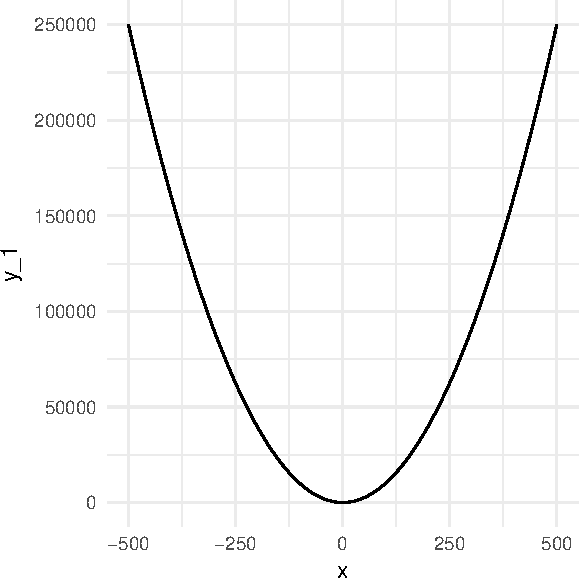
\includegraphics{Optimization_files/figure-latex/FOC_dim_1-1} \end{center}

In more than one dimension:

\begin{Shaded}
\begin{Highlighting}[]
\NormalTok{x_}\DecValTok{1}\NormalTok{ <-}\StringTok{ }\NormalTok{x_}\DecValTok{2}\NormalTok{ <-}\StringTok{ }\KeywordTok{seq}\NormalTok{(}\OperatorTok{-}\DecValTok{5}\NormalTok{, }\DecValTok{5}\NormalTok{, }\FloatTok{0.20}\NormalTok{)}

\NormalTok{z_plus <-}\StringTok{ }\KeywordTok{outer}\NormalTok{(x_}\DecValTok{1}\NormalTok{, x_}\DecValTok{2}\NormalTok{, }
                \DataTypeTok{FUN =} \ControlFlowTok{function}\NormalTok{(x_}\DecValTok{1}\NormalTok{,x_}\DecValTok{2}\NormalTok{)\{x_}\DecValTok{1}\OperatorTok{^}\DecValTok{2}\OperatorTok{+}\NormalTok{x_}\DecValTok{2}\OperatorTok{^}\DecValTok{2}\NormalTok{\}}
\NormalTok{                )}
\NormalTok{z_minus <-}\StringTok{ }\KeywordTok{outer}\NormalTok{(x_}\DecValTok{1}\NormalTok{, x_}\DecValTok{2}\NormalTok{,}
                 \DataTypeTok{FUN =} \ControlFlowTok{function}\NormalTok{(x_}\DecValTok{1}\NormalTok{,x_}\DecValTok{2}\NormalTok{)\{}\OperatorTok{-}\NormalTok{x_}\DecValTok{1}\OperatorTok{^}\DecValTok{2}\OperatorTok{-}\NormalTok{x_}\DecValTok{2}\OperatorTok{^}\DecValTok{2}\NormalTok{\}}
\NormalTok{                 )}

\KeywordTok{persp}\NormalTok{(x_}\DecValTok{1}\NormalTok{, x_}\DecValTok{2}\NormalTok{, z_plus, }\DataTypeTok{theta =} \DecValTok{60}\NormalTok{, }\DataTypeTok{phi =} \DecValTok{0}\NormalTok{)}
\end{Highlighting}
\end{Shaded}

\begin{center}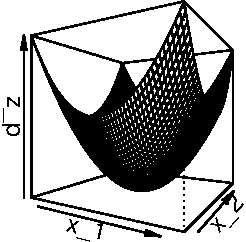
\includegraphics{Optimization_files/figure-latex/FOC_dim_2-1} \end{center}

\begin{Shaded}
\begin{Highlighting}[]
\KeywordTok{persp}\NormalTok{(x_}\DecValTok{1}\NormalTok{, x_}\DecValTok{2}\NormalTok{, z_minus, }\DataTypeTok{theta =} \DecValTok{60}\NormalTok{, }\DataTypeTok{phi =} \DecValTok{0}\NormalTok{)}
\end{Highlighting}
\end{Shaded}

\begin{center}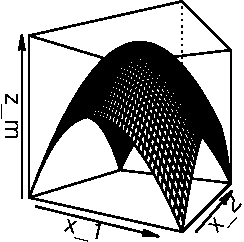
\includegraphics{Optimization_files/figure-latex/FOC_dim_2-2} \end{center}

End points or corner points are generally not considered critical points
though they can contain extreme points. (For the plot \(f(x)=x^2\) what
is/are maximal points if \(x\in [l, b]\)?) Conventionally, critical
points are thought to be points interior to the domain.

Functions can be separated into classes on the basis of how
differentiable they are (the differentiability class). For example, all
functions that are continuous form the \(C^0\) class; those that are
differentiable and their derivatives also continuous form the class
\(C^1\); those whose second derivatives are continuous form the class
\(C^2\) and so on.\footnote{A function is ``smooth'' if all derivatives
  are continous: \(f\in C^{\infty}\); and analytical
  \(f \in C^{\omega}\) if it is smooth \emph{and} its Taylor
  approximation converges to its function value at all points in the
  domain.}

\textbf{Theorem:} If \(x^*\in \mathbb{R}^n\) is an interior point in the
domain of the real-valued function \(F\in C^1\), then it is a critical
point when \[
  \frac{\partial F}{\partial x_i}(x^*) = 0, i\in \{1, 2,\hdots, n\}
\]

\subsection{Second Order Conditions}\label{second-order-conditions}

Critical points are interior points at which all first partial
derivatives are 0. However, this in itself is not enough for us to know
if the critical point is a maximum, a minimum or neither. For this, we
need to consider its second derivatives.

For the function \(F\in C^2, x\in U\subset \mathbb{R}^n\), (\(U\) is
open in \(\mathbb{R}^n\)) the \emph{Hessian} is the following second
derivative matrix: \[
D^2F(x^*) = \begin{bmatrix}
\frac{\partial F}{\partial x_1^2}(x^*) & \hdots &\frac{\partial F}{\partial x_n\partial x_1}(x^*)\\
\vdots & \ddots & \vdots\\
\frac{\partial F}{\partial x_1\partial x_n}(x^*) & \hdots & \frac{\partial F}{\partial x_n^2}(x^*)
\end{bmatrix}
\]

Since for the function \(F\in C^2\), the cross-partials
\(\frac{\partial F}{\partial x_i \partial x_j} = \frac{\partial F}{\partial x_j \partial x_i}\),
the Hessian is symmetric.

The second order conditions are based on the Hessian. Just as in the one
dimensional case, where there occurs a maximum at a critical point if
the second derivative is negative; there occurs a maximum at the
critical point \(x^*\in U\subset \mathbb{R}^n\) if the Hessian is
\emph{negative definite}.

\textbf{Theorem:} For the function
\(F\in C^2, x\in U\subset \mathbb{R}^n\) with critical point \(x^*\):

\begin{enumerate}
\def\labelenumi{\arabic{enumi}.}
\tightlist
\item
  If the Hessian \(D^2F(x^*)\) is negative definite, then \(x^*\) is a
  local maximum.
\item
  If the Hessian \(D^2F(x^*)\) is positive definite, then \(x^*\) is a
  local minimum.
\item
  If the Hessian \(D^2F(x^*)\) is indefinite, then \(x^*\) is neither.
  (\(x^*\) is a ``saddle point''.)
\end{enumerate}

\subsection{Convex Functions and Global
Minima}\label{convex-functions-and-global-minima}

While the conditions above classify critical points as maximal, minimal
or saddle; these are only local optima. However if we consider only a
special class of functions called \emph{convex}, we can guarantee that
the local minimum will also be the global minimum!

A simple example of a convex function is \(f(x) = x^2\). It has one
minimum at \(x=0\) which is also its global minimum. The added wrinkle
is that the domain of a convex function must be a \emph{convex} set.

\subsubsection{Convex Set}\label{convex-set}

A set \(U\subset \mathbb{R}^n\) is convex if for two points in it, the
whole line connecting the two points must also fully lie in \(U\). More
formally, a set \(U\) is convex if \(\forall t\in[0,1]\) \[
x, y \in U \Rightarrow tx+(1-t)y\in U
\] (Can you see this geometrically?)

\subsubsection{Convex Function}\label{convex-function}

Now, we can define a convex \emph{function} whose domain is a convex
\emph{set} by stipulating that the image of the line connecting \(x\) to
\(y\) lie below the line itself. Hence a function \(F\) is convex if its
domain \(U\in \mathbb{R}^n\) is convex; and for all \(x, y\in U\) and
\(\forall t\in[0,1]\) \[
tF(x) + (1-t)F(y) \geq F(tx + (1-t)y)
\]

We can check if this condition is satisfied for our one dimensional
convex function \(f(x)=x^2\).

\begin{Shaded}
\begin{Highlighting}[]
\NormalTok{plot_x_square }\OperatorTok{+}\StringTok{ }
\StringTok{  }\KeywordTok{geom_segment}\NormalTok{(}\KeywordTok{aes}\NormalTok{(}\DataTypeTok{x =} \DecValTok{0}\NormalTok{, }
                   \DataTypeTok{y =} \DecValTok{0}\NormalTok{, }
                   \DataTypeTok{xend =} \DecValTok{400}\NormalTok{, }
                   \DataTypeTok{yend =} \DecValTok{400}\OperatorTok{^}\DecValTok{2}
\NormalTok{                   ), }
               \DataTypeTok{linetype =} \StringTok{"dotdash"}\NormalTok{, }
               \DataTypeTok{color =} \StringTok{"red"}
\NormalTok{               )}
\end{Highlighting}
\end{Shaded}

\begin{center}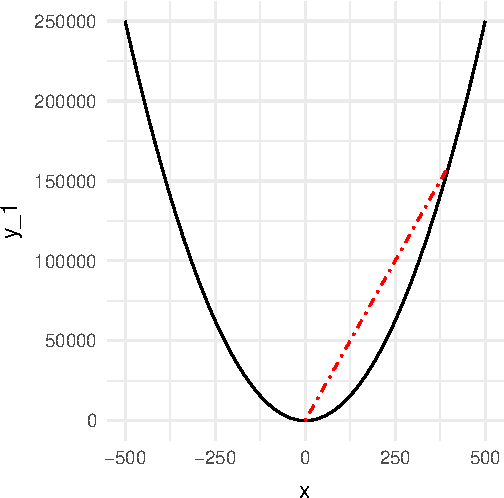
\includegraphics{Optimization_files/figure-latex/func_convex-1} \end{center}

\subsubsection{Concave Function}\label{concave-function}

A \emph{concave} function is simply the negative of a convex function.
In one dimension, \(-x^2, \log(x), \sqrt{x}\) etc. are some commonly
known concave functions. For these, local maxima are global maxima. Note
that just like the convex functions, domains of concave functions must
be convex too.

\textbf{Theorem:} If \(F:U \to \mathbb{R}\), (where
\(U\subset \mathbb{R}^n\) is convex and open) \(F\in C^2\) and convex
then

\begin{enumerate}
\def\labelenumi{\arabic{enumi}.}
\tightlist
\item
  \(D^2F(x)\) is positive semidefinite for \(x\in U\)
\item
  \(F(y)-F(x)\geq DF(x)\cdot(y-x)\) for \(x, y\in U\)
\item
  If for \(x^*\in U, DF(x^*)=0\) then \(x^*\) is the global minimum
\end{enumerate}

\section{Computation: Unconstrained
Optimization}\label{computation-unconstrained-optimization}

There are several special packages written in \texttt{R} for solving
optimization problems. A core set of packages is included with the
installation of \texttt{R}, with more than 12,500 additional packages
(as of May 2018) available at the ``Comprehensive R Archive Network''
(CRAN). Additionally, packages related to a topic, say, Econometrics or
Optimization or Differential Equations etc. can be found by looking them
up in CRAN Task Views: \url{https://cran.r-project.org/web/views/}.

We quote here from CRAN Task Views: Optimization

\begin{quote}
For one-dimensional unconstrained function optimization there is
\texttt{optimize()} which searches an interval for a minimum or maximum.
Function \texttt{optim()} provides an implementation of the
Broyden-Fletcher-Goldfarb-Shanno (BFGS) method, bounded BFGS, conjugate
gradient (CG), Nelder-Mead, and simulated annealing (SANN) optimization
methods. It utilizes gradients, if provided, for faster convergence.
Typically it is used for unconstrained optimization but includes an
option for box-constrained optimization.
\end{quote}

\subsection{One-Dimension}\label{one-dimension}

The \texttt{optimize()} function is used for one dimensional problems.
Its first argument is the function to be optimized and the second
argument is the solution search space as provided by the user. It may
only be used to detect local extrema.

To illustrate, consider \(xsin(4x)\):

\begin{Shaded}
\begin{Highlighting}[]
\CommentTok{# Another function for optimization}
\NormalTok{func_2_x <-}\StringTok{ }\ControlFlowTok{function}\NormalTok{(x) \{x}\OperatorTok{*}\KeywordTok{sin}\NormalTok{(}\DecValTok{4}\OperatorTok{*}\NormalTok{x)\}}

\KeywordTok{curve}\NormalTok{(func_2_x, }\OperatorTok{-}\DecValTok{1}\NormalTok{, }\DecValTok{3}\NormalTok{) }\CommentTok{#note base R graphics function curve()}
\end{Highlighting}
\end{Shaded}

\begin{center}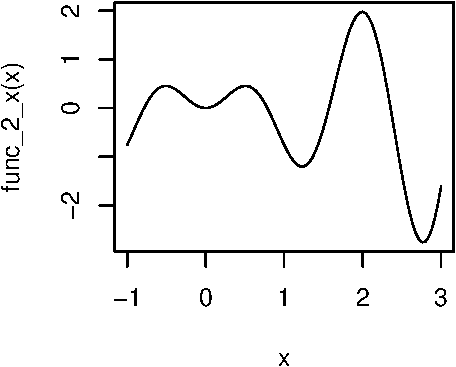
\includegraphics{Optimization_files/figure-latex/opt_unconstr_optimize-1} \end{center}

\begin{Shaded}
\begin{Highlighting}[]
\CommentTok{# Via ggplot()}
\NormalTok{x <-}\StringTok{ }\KeywordTok{seq}\NormalTok{(}\OperatorTok{-}\DecValTok{1}\NormalTok{, }\DecValTok{3}\NormalTok{, }\FloatTok{0.01}\NormalTok{)}
\NormalTok{y <-}\StringTok{ }\KeywordTok{func_2_x}\NormalTok{(x)}
\NormalTok{data_plot_gg <-}\StringTok{ }\KeywordTok{cbind}\NormalTok{(x, y) }\OperatorTok\StringTok{ }\NormalTok{tibble}\OperatorTok{::}\KeywordTok{as_tibble}\NormalTok{()}

\KeywordTok{ggplot}\NormalTok{(data_plot_gg, }\KeywordTok{aes}\NormalTok{(x, y)) }\OperatorTok{+}
\StringTok{  }\KeywordTok{geom_line}\NormalTok{() }\OperatorTok{+}
\StringTok{  }\KeywordTok{theme_minimal}\NormalTok{()}
\end{Highlighting}
\end{Shaded}

\begin{center}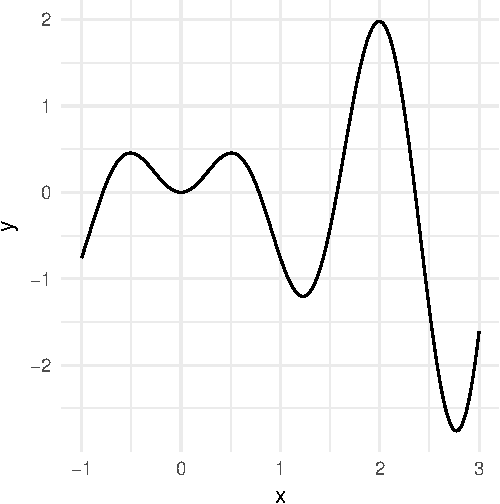
\includegraphics{Optimization_files/figure-latex/opt_unconstr_optimize-2} \end{center}

\begin{Shaded}
\begin{Highlighting}[]
\CommentTok{# Using optimize()}
\NormalTok{(optim_min_mult <-}\StringTok{ }\KeywordTok{optimize}\NormalTok{(}\DataTypeTok{f =}\NormalTok{ func_2_x, }
                            \DataTypeTok{interval =} \KeywordTok{c}\NormalTok{(}\DecValTok{0}\NormalTok{, }\DecValTok{3}\NormalTok{)}
\NormalTok{                            ) }\CommentTok{#default = minimum}
\NormalTok{) }
\end{Highlighting}
\end{Shaded}

\begin{verbatim}
## $minimum
## [1] 1.228297
## 
## $objective
## [1] -1.203617
\end{verbatim}

It seems from the plot of \(xsin(4x)\) that the local minimum is at
around 1.2 and the global minimum is at around 2.8. However, our
invocation of the \texttt{optimize()} function yields a minimum of
1.2282971, which is not the global minimum even though it lies within
our set search limits (\(2.8\in c(0,3)\)). This is so because the
function \texttt{optimize()} returns the first minimum it encounters in
the search algorithm. Since we can observe the plot, we should supply a
better default search region to capture the global minimum:

\begin{Shaded}
\begin{Highlighting}[]
\KeywordTok{optimize}\NormalTok{(func_2_x, }\KeywordTok{c}\NormalTok{(}\FloatTok{1.5}\NormalTok{, }\DecValTok{3}\NormalTok{))}
\end{Highlighting}
\end{Shaded}

\begin{verbatim}
## $minimum
## [1] 2.771403
## 
## $objective
## [1] -2.760177
\end{verbatim}

In order to find the maximum:

\begin{Shaded}
\begin{Highlighting}[]
\KeywordTok{optimize}\NormalTok{(func_2_x, }\KeywordTok{c}\NormalTok{(}\FloatTok{1.5}\NormalTok{, }\DecValTok{3}\NormalTok{), }\DataTypeTok{maximum =} \OtherTok{TRUE}\NormalTok{)}
\end{Highlighting}
\end{Shaded}

\begin{verbatim}
## $maximum
## [1] 1.994653
## 
## $objective
## [1] 1.979182
\end{verbatim}

The \texttt{optimize()} function works with non-differentiable functions
too:

\begin{Shaded}
\begin{Highlighting}[]
\NormalTok{func_3_x <-}\StringTok{ }\ControlFlowTok{function}\NormalTok{(x) \{}\KeywordTok{abs}\NormalTok{(x}\OperatorTok{-}\DecValTok{1}\NormalTok{)}\OperatorTok{+}\DecValTok{2}\OperatorTok{*}\KeywordTok{abs}\NormalTok{(x}\OperatorTok{-}\DecValTok{2}\NormalTok{)\}}

\KeywordTok{plot}\NormalTok{(func_3_x, }\OperatorTok{-}\DecValTok{1}\NormalTok{, }\DecValTok{4}\NormalTok{) }\CommentTok{#note generic function plotting in base R}
\end{Highlighting}
\end{Shaded}

\begin{center}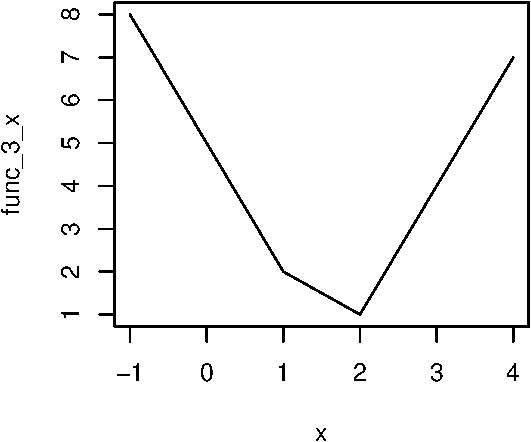
\includegraphics{Optimization_files/figure-latex/optimize_non_diff-1} \end{center}

\begin{Shaded}
\begin{Highlighting}[]
\CommentTok{# Via ggplot}
\NormalTok{x_}\DecValTok{3}\NormalTok{ <-}\StringTok{ }\KeywordTok{seq}\NormalTok{(}\OperatorTok{-}\DecValTok{1}\NormalTok{, }\DecValTok{4}\NormalTok{, }\FloatTok{0.01}\NormalTok{)}
\NormalTok{y_}\DecValTok{3}\NormalTok{ <-}\StringTok{ }\KeywordTok{func_3_x}\NormalTok{(x_}\DecValTok{3}\NormalTok{)}

\KeywordTok{ggplot}\NormalTok{(tibble}\OperatorTok{::}\KeywordTok{as_tibble}\NormalTok{(}\KeywordTok{cbind}\NormalTok{(x_}\DecValTok{3}\NormalTok{,y_}\DecValTok{3}\NormalTok{)),}
       \KeywordTok{aes}\NormalTok{(x_}\DecValTok{3}\NormalTok{, y_}\DecValTok{3}\NormalTok{)}
\NormalTok{       ) }\OperatorTok{+}\StringTok{ }
\StringTok{  }\KeywordTok{geom_line}\NormalTok{() }\OperatorTok{+}
\StringTok{  }\KeywordTok{theme_minimal}\NormalTok{()}
\end{Highlighting}
\end{Shaded}

\begin{center}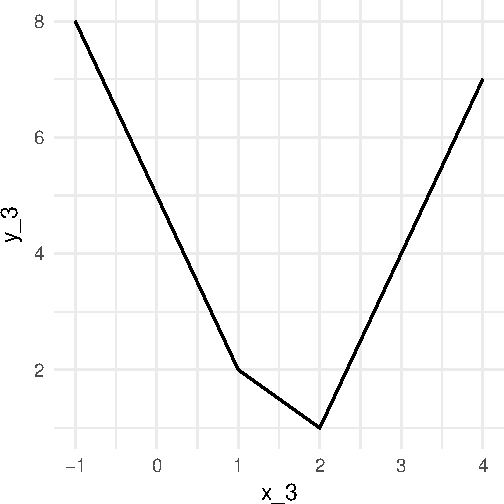
\includegraphics{Optimization_files/figure-latex/optimize_non_diff-2} \end{center}

\begin{Shaded}
\begin{Highlighting}[]
\NormalTok{(optim_x_}\DecValTok{3}\NormalTok{ <-}\StringTok{ }\KeywordTok{optimize}\NormalTok{(func_3_x, }\KeywordTok{c}\NormalTok{(}\DecValTok{0}\NormalTok{,}\DecValTok{3}\NormalTok{)))}
\end{Highlighting}
\end{Shaded}

\begin{verbatim}
## $minimum
## [1] 1.999991
## 
## $objective
## [1] 1.000009
\end{verbatim}

\subsection{Multidimensional
Programming}\label{multidimensional-programming}

We use the package \texttt{optim()} for solving multidimensional
programs.

\begin{Shaded}
\begin{Highlighting}[]
\KeywordTok{optim}\NormalTok{(}\DataTypeTok{par =}\NormalTok{ ..., }\CommentTok{#initial value vector (parameters)}
      \DataTypeTok{fn =}\NormalTok{ ..., }\CommentTok{#objective function (minimization)}
      \DataTypeTok{lower =} \OperatorTok{-}\OtherTok{Inf}\NormalTok{, }\CommentTok{#lower bound}
      \DataTypeTok{upper =} \OtherTok{Inf}\NormalTok{, }\CommentTok{#upper bound}
      \DataTypeTok{method =} \StringTok{''}\NormalTok{, }\CommentTok{#default method = "Nelder-Mead"}
      \DataTypeTok{control =}\NormalTok{ ..., }\CommentTok{#maximum iterations}
\NormalTok{      )}
\end{Highlighting}
\end{Shaded}

Consider the function \(f(x) = 2(x_1-1)^2+5(x_2-3)^2+10\)

\begin{Shaded}
\begin{Highlighting}[]
\NormalTok{func_optim <-}\StringTok{ }\ControlFlowTok{function}\NormalTok{(x)}
\NormalTok{\{}
  \DecValTok{2}\OperatorTok{*}\NormalTok{(x[}\DecValTok{1}\NormalTok{]}\OperatorTok{-}\DecValTok{1}\NormalTok{)}\OperatorTok{^}\DecValTok{2} \OperatorTok{+}\StringTok{ }\DecValTok{5}\OperatorTok{*}\NormalTok{(x[}\DecValTok{2}\NormalTok{]}\OperatorTok{-}\DecValTok{3}\NormalTok{)}\OperatorTok{^}\DecValTok{2} \OperatorTok{+}\StringTok{ }\DecValTok{10}
\NormalTok{\}}

\NormalTok{optim_min <-}\StringTok{ }\KeywordTok{optim}\NormalTok{(}\KeywordTok{c}\NormalTok{(}\DecValTok{1}\NormalTok{,}\DecValTok{1}\NormalTok{), func_optim) }\CommentTok{#x=(x_1,x_2)=c(1,1)}
\KeywordTok{print}\NormalTok{(optim_min)}
\end{Highlighting}
\end{Shaded}

\begin{verbatim}
## $par
## [1] 1.000168 3.000232
## 
## $value
## [1] 10
## 
## $counts
## function gradient 
##       75       NA 
## 
## $convergence
## [1] 0
## 
## $message
## NULL
\end{verbatim}

Another example:
\(f(x) = \frac{1}{x_1}+\frac{1}{x_2}+\frac{1-x_2}{x_2(1-x_1)}+\frac{1}{(1-x_1)(1-x_2)}\)

\begin{Shaded}
\begin{Highlighting}[]
\NormalTok{func_optim_}\DecValTok{2}\NormalTok{ <-}\StringTok{ }\ControlFlowTok{function}\NormalTok{(x1, x2) }
\NormalTok{\{}
  \KeywordTok{return}\NormalTok{(}\DecValTok{1}\OperatorTok{/}\NormalTok{x1 }\OperatorTok{+}\StringTok{ }\DecValTok{1}\OperatorTok{/}\NormalTok{x2 }\OperatorTok{+}\StringTok{ }
\StringTok{    }\NormalTok{(}\DecValTok{1}\OperatorTok{-}\NormalTok{x2)}\OperatorTok{/}\NormalTok{(x2}\OperatorTok{*}\NormalTok{(}\DecValTok{1}\OperatorTok{-}\NormalTok{x1)) }\OperatorTok{+}\StringTok{ }
\StringTok{    }\DecValTok{1}\OperatorTok{/}\NormalTok{((}\DecValTok{1}\OperatorTok{-}\NormalTok{x1)}\OperatorTok{*}\NormalTok{(}\DecValTok{1}\OperatorTok{-}\NormalTok{x2))}
\NormalTok{    )}
\NormalTok{\}}

\NormalTok{x_}\DecValTok{1}\NormalTok{ <-}\StringTok{ }\NormalTok{x_}\DecValTok{2}\NormalTok{ <-}\StringTok{ }\KeywordTok{seq}\NormalTok{(}\FloatTok{0.1}\NormalTok{, }\FloatTok{0.9}\NormalTok{, }\FloatTok{0.02}\NormalTok{)}
\NormalTok{z <-}\StringTok{ }\KeywordTok{outer}\NormalTok{(x_}\DecValTok{1}\NormalTok{, x_}\DecValTok{2}\NormalTok{, }\DataTypeTok{FUN =} \StringTok{"func_optim_2"}\NormalTok{)}

\CommentTok{# Different perspectives}
\KeywordTok{persp}\NormalTok{(x_}\DecValTok{1}\NormalTok{, x_}\DecValTok{2}\NormalTok{, z, }\DataTypeTok{theta =} \DecValTok{45}\NormalTok{, }\DataTypeTok{phi =} \DecValTok{0}\NormalTok{) }
\end{Highlighting}
\end{Shaded}

\begin{center}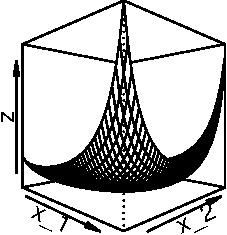
\includegraphics{Optimization_files/figure-latex/opt_unconstr_optim_2-1} \end{center}

\begin{Shaded}
\begin{Highlighting}[]
\KeywordTok{persp}\NormalTok{(x_}\DecValTok{1}\NormalTok{, x_}\DecValTok{2}\NormalTok{, z, }\DataTypeTok{theta =} \DecValTok{0}\NormalTok{, }\DataTypeTok{phi =} \DecValTok{45}\NormalTok{)}
\end{Highlighting}
\end{Shaded}

\begin{center}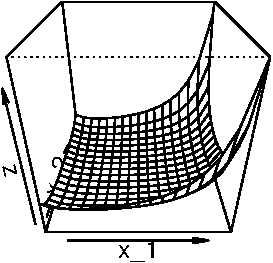
\includegraphics{Optimization_files/figure-latex/opt_unconstr_optim_2-2} \end{center}

\begin{Shaded}
\begin{Highlighting}[]
\KeywordTok{persp}\NormalTok{(x_}\DecValTok{1}\NormalTok{, x_}\DecValTok{2}\NormalTok{, z, }\DataTypeTok{theta =} \OperatorTok{-}\DecValTok{45}\NormalTok{, }\DataTypeTok{phi =} \DecValTok{0}\NormalTok{)}
\end{Highlighting}
\end{Shaded}

\begin{center}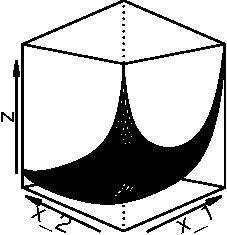
\includegraphics{Optimization_files/figure-latex/opt_unconstr_optim_2-3} \end{center}

\begin{Shaded}
\begin{Highlighting}[]
\NormalTok{func_opt_}\DecValTok{2}\NormalTok{ <-}\StringTok{ }\ControlFlowTok{function}\NormalTok{(x)}
\NormalTok{\{}
\NormalTok{  x1 <-}\StringTok{ }\NormalTok{x[}\DecValTok{1}\NormalTok{]}
\NormalTok{  x2 <-}\StringTok{ }\NormalTok{x[}\DecValTok{2}\NormalTok{]}
  \KeywordTok{return}\NormalTok{((}\DecValTok{1}\OperatorTok{/}\NormalTok{x1 }\OperatorTok{+}\StringTok{ }\DecValTok{1}\OperatorTok{/}\NormalTok{x2 }\OperatorTok{+}\StringTok{ }
\StringTok{            }\NormalTok{(}\DecValTok{1}\OperatorTok{-}\NormalTok{x2)}\OperatorTok{/}\NormalTok{(x2}\OperatorTok{*}\NormalTok{(}\DecValTok{1}\OperatorTok{-}\NormalTok{x1)) }\OperatorTok{+}\StringTok{ }
\StringTok{            }\DecValTok{1}\OperatorTok{/}\NormalTok{((}\DecValTok{1}\OperatorTok{-}\NormalTok{x1)}\OperatorTok{*}\NormalTok{(}\DecValTok{1}\OperatorTok{-}\NormalTok{x2)))}
\NormalTok{         )}
\NormalTok{\}}

\KeywordTok{optim}\NormalTok{(}\KeywordTok{c}\NormalTok{(}\FloatTok{0.5}\NormalTok{, }\FloatTok{0.5}\NormalTok{), func_opt_}\DecValTok{2}\NormalTok{)}
\end{Highlighting}
\end{Shaded}

\begin{verbatim}
## $par
## [1] 0.3636913 0.5612666
## 
## $value
## [1] 9.341785
## 
## $counts
## function gradient 
##       55       NA 
## 
## $convergence
## [1] 0
## 
## $message
## NULL
\end{verbatim}

\section{Application: Maximum Likelihood
Estimation}\label{application-maximum-likelihood-estimation}

While informally the words `probability' and `likelihood' can be used
somewhat interchangeably, in statistics there is an important difference
between the two. Probability is the plausibility of an event happening
given certain model parameter values; while likelihood is the
plausibility of the model parameter values given certain observed
events.\footnote{Tellingly, the likelihoods, when added, do not need to
  add up to 1 unlike probabilities.}

\textbf{Illustration:} Suppose we flip a coin where \(p_H\) denotes the
probability of being heads. Suppose we get two heads in a row. Suppose
we assume the coin flips are independent and identically distributed.
Then

\[\Pr(\{H,H\}|p_H = 0.5) = 0.5\cdot0.5=0.25= \mathcal{L}(p_H=0.5|\{H,H\})\]

More formally, for the ``likelihood function'' \(\mathcal{L}(\cdot)\)

\[\text{Pr}_{\theta}(X = x) := \mathcal{L}(\theta|X = x)\] or for
continuous random variables \(X\),

\[f_{\theta}(x) := \mathcal{L}(\theta|X=x)\]

Since we care most about the point in the domain where the likelihood
reaches its maximum, we often compute the \emph{log}-likelihood
\(l(\cdot)=\ln(\mathcal{L}(\cdot))\) since the logarithm is strictly
increasing function and therefore must possess the same argmax.

The maximum likelihood estimate is:
\[\hat{\theta}\in\{\text{argmax}_{\theta\in \Theta} \mathcal{L}(\theta; x)\}\]

For some models, MLEs have closed forms. For many others no closed-form
solutions to the maximization problem is known; and for many others,
there may be multiple solutions or no solutions.

If samples are independent and identically distributed:

\[\hat{l}(\theta; x) = \max{} \frac{1}{n}\sum_{i=1}^n \ln(f(x_i|\theta))\]

Note that this is the sample analogue of maximimzing the expected
log-likelihood: \(\max{} \mathbb{E}[\ln(f(x_i|\theta))]\).

\subsection{Computation: Maximum
Likelihood}\label{computation-maximum-likelihood}

Suppose for a normal random variable \(X\sim \mathcal{N}(\mu,\sigma)\)
there are iid observations \(\{x_i\}_{i=1}^n\). Then the log-likelihood
function is:
\[l(\mu, \sigma)=\sum_{i = 1}^n \ln(f(x_i)|\theta=(\mu, \sigma))\]
\[l(\mu, \sigma)=-\frac{n}{2}\ln(2\pi)-\frac{n}{2}\ln(\sigma^2)-
\frac{1}{2\sigma^2}\sum_{i=1}^n (x_i-\mu)^2\]

Taking first order conditions with respect to \(\mu\) and \(\sigma^2\)
yields maximum likelihood estimates
\[\hat{\mu} = \bar{x} = \frac{1}{n}\sum_{i=1}^n x_i\]
\[\widehat{\sigma^2} = \frac{1}{n}\sum_{i=1}^n (x_i-\bar{x})^2\]

Let's check if we get the same results with the \texttt{optim()}
function

\begin{Shaded}
\begin{Highlighting}[]
\NormalTok{x_vec <-}\StringTok{ }\KeywordTok{rnorm}\NormalTok{(}\DecValTok{1000}\NormalTok{, }\DecValTok{5}\NormalTok{, }\DecValTok{2}\NormalTok{) }\CommentTok{#1000 normals with mean 5 and sigma 2}

\NormalTok{neg_log_likeli <-}\StringTok{ }\ControlFlowTok{function}\NormalTok{(theta)}
\NormalTok{\{}
\NormalTok{  n <-}\StringTok{ }\KeywordTok{length}\NormalTok{(x_vec)}
\NormalTok{  NLL <-}\StringTok{ }\KeywordTok{sum}\NormalTok{((x_vec }\OperatorTok{-}\StringTok{ }\NormalTok{theta[}\DecValTok{1}\NormalTok{])}\OperatorTok{^}\DecValTok{2}\NormalTok{)}\OperatorTok{/}\NormalTok{(}\DecValTok{2}\OperatorTok{*}\NormalTok{theta[}\DecValTok{2}\NormalTok{]) }\OperatorTok{+}\StringTok{ }
\StringTok{    }\NormalTok{(n}\OperatorTok{/}\DecValTok{2}\NormalTok{)}\OperatorTok{*}\KeywordTok{log}\NormalTok{(theta[}\DecValTok{2}\NormalTok{])}
  
  \KeywordTok{return}\NormalTok{(NLL)}
\NormalTok{\}}

\KeywordTok{optim}\NormalTok{(theta <-}\StringTok{ }\KeywordTok{c}\NormalTok{(}\DecValTok{0}\NormalTok{,}\DecValTok{1}\NormalTok{), }\CommentTok{#(0,1) starting}
\NormalTok{      neg_log_likeli, }
      \DataTypeTok{hessian=}\OtherTok{TRUE} \CommentTok{#print the Hessian matrix}
\NormalTok{      ) }
\end{Highlighting}
\end{Shaded}

\begin{verbatim}
## $par
## [1] 5.084675 4.163636
## 
## $value
## [1] 1213.22
## 
## $counts
## function gradient 
##       81       NA 
## 
## $convergence
## [1] 0
## 
## $message
## NULL
## 
## $hessian
##              [,1]        [,2]
## [1,] 240.17470344 -0.06452115
## [2,]  -0.06452115 28.84493057
\end{verbatim}

\begin{Shaded}
\begin{Highlighting}[]
\KeywordTok{optim}\NormalTok{(theta <-}\StringTok{ }\KeywordTok{c}\NormalTok{(}\FloatTok{0.5}\NormalTok{,}\FloatTok{1.2}\NormalTok{), }\CommentTok{#different starting point}
\NormalTok{      neg_log_likeli, }
      \DataTypeTok{hessian=}\OtherTok{TRUE}
\NormalTok{      ) }
\end{Highlighting}
\end{Shaded}

\begin{verbatim}
## $par
## [1] 5.083225 4.165530
## 
## $value
## [1] 1213.22
## 
## $counts
## function gradient 
##       79       NA 
## 
## $convergence
## [1] 0
## 
## $message
## NULL
## 
## $hessian
##              [,1]        [,2]
## [1,] 240.06549381  0.01912008
## [2,]   0.01912008 28.79248171
\end{verbatim}

\begin{Shaded}
\begin{Highlighting}[]
\KeywordTok{mean}\NormalTok{(x_vec)}
\end{Highlighting}
\end{Shaded}

\begin{verbatim}
## [1] 5.083557
\end{verbatim}

\begin{Shaded}
\begin{Highlighting}[]
\KeywordTok{sd}\NormalTok{(x_vec)}
\end{Highlighting}
\end{Shaded}

\begin{verbatim}
## [1] 2.041572
\end{verbatim}


\end{document}
